\section{Grachten}

Problem summary: given three lengths $AB$, $AC$, $BD$ forming the base and
partial lengths for the adjacent side and hypotenuse, determine the remaining
length of the adjacent side.

\begin{center}
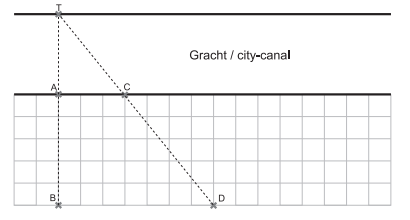
\includegraphics[scale=0.75]{f_diagram.png}
\end{center}

Let the goal length be known as $x$. We use similar triangles to work out the
correct size of $x$ from the givens:

\begin{align*}
  \frac{x}{AC} &= \frac{x+AB}{BD}             \\[3mm]
  x \times BD &= x \times AC + AB \times AC   \\[3mm]
  x &= \frac{AB \times AC}{BD - AC}
\end{align*}

We simplify the fraction with the GCD and we're done.

\vspace{0.5cm}
Overall this runs in $O(\log 1000)$ time because of the GCD and $O(1)$ memory.
